% GNUPLOT: LaTeX picture with Postscript
\begingroup
  \makeatletter
  \providecommand\color[2][]{%
    \GenericError{(gnuplot) \space\space\space\@spaces}{%
      Package color not loaded in conjunction with
      terminal option `colourtext'%
    }{See the gnuplot documentation for explanation.%
    }{Either use 'blacktext' in gnuplot or load the package
      color.sty in LaTeX.}%
    \renewcommand\color[2][]{}%
  }%
  \providecommand\includegraphics[2][]{%
    \GenericError{(gnuplot) \space\space\space\@spaces}{%
      Package graphicx or graphics not loaded%
    }{See the gnuplot documentation for explanation.%
    }{The gnuplot epslatex terminal needs graphicx.sty or graphics.sty.}%
    \renewcommand\includegraphics[2][]{}%
  }%
  \providecommand\rotatebox[2]{#2}%
  \@ifundefined{ifGPcolor}{%
    \newif\ifGPcolor
    \GPcolortrue
  }{}%
  \@ifundefined{ifGPblacktext}{%
    \newif\ifGPblacktext
    \GPblacktexttrue
  }{}%
  % define a \g@addto@macro without @ in the name:
  \let\gplgaddtomacro\g@addto@macro
  % define empty templates for all commands taking text:
  \gdef\gplbacktext{}%
  \gdef\gplfronttext{}%
  \makeatother
  \ifGPblacktext
    % no textcolor at all
    \def\colorrgb#1{}%
    \def\colorgray#1{}%
  \else
    % gray or color?
    \ifGPcolor
      \def\colorrgb#1{\color[rgb]{#1}}%
      \def\colorgray#1{\color[gray]{#1}}%
      \expandafter\def\csname LTw\endcsname{\color{white}}%
      \expandafter\def\csname LTb\endcsname{\color{black}}%
      \expandafter\def\csname LTa\endcsname{\color{black}}%
      \expandafter\def\csname LT0\endcsname{\color[rgb]{1,0,0}}%
      \expandafter\def\csname LT1\endcsname{\color[rgb]{0,1,0}}%
      \expandafter\def\csname LT2\endcsname{\color[rgb]{0,0,1}}%
      \expandafter\def\csname LT3\endcsname{\color[rgb]{1,0,1}}%
      \expandafter\def\csname LT4\endcsname{\color[rgb]{0,1,1}}%
      \expandafter\def\csname LT5\endcsname{\color[rgb]{1,1,0}}%
      \expandafter\def\csname LT6\endcsname{\color[rgb]{0,0,0}}%
      \expandafter\def\csname LT7\endcsname{\color[rgb]{1,0.3,0}}%
      \expandafter\def\csname LT8\endcsname{\color[rgb]{0.5,0.5,0.5}}%
    \else
      % gray
      \def\colorrgb#1{\color{black}}%
      \def\colorgray#1{\color[gray]{#1}}%
      \expandafter\def\csname LTw\endcsname{\color{white}}%
      \expandafter\def\csname LTb\endcsname{\color{black}}%
      \expandafter\def\csname LTa\endcsname{\color{black}}%
      \expandafter\def\csname LT0\endcsname{\color{black}}%
      \expandafter\def\csname LT1\endcsname{\color{black}}%
      \expandafter\def\csname LT2\endcsname{\color{black}}%
      \expandafter\def\csname LT3\endcsname{\color{black}}%
      \expandafter\def\csname LT4\endcsname{\color{black}}%
      \expandafter\def\csname LT5\endcsname{\color{black}}%
      \expandafter\def\csname LT6\endcsname{\color{black}}%
      \expandafter\def\csname LT7\endcsname{\color{black}}%
      \expandafter\def\csname LT8\endcsname{\color{black}}%
    \fi
  \fi
    \setlength{\unitlength}{0.0500bp}%
    \ifx\gptboxheight\undefined%
      \newlength{\gptboxheight}%
      \newlength{\gptboxwidth}%
      \newsavebox{\gptboxtext}%
    \fi%
    \setlength{\fboxrule}{0.5pt}%
    \setlength{\fboxsep}{1pt}%
\begin{picture}(4740.00,2880.00)%
    \gplgaddtomacro\gplbacktext{%
      \colorrgb{0.27,0.27,0.27}%
      \put(455,558){\makebox(0,0)[r]{\strut{}\scriptsize{$10^{-5}$}}}%
      \colorrgb{0.27,0.27,0.27}%
      \put(455,948){\makebox(0,0)[r]{\strut{}\scriptsize{$10^{-4}$}}}%
      \colorrgb{0.27,0.27,0.27}%
      \put(455,1338){\makebox(0,0)[r]{\strut{}\scriptsize{$10^{-3}$}}}%
      \colorrgb{0.27,0.27,0.27}%
      \put(455,1727){\makebox(0,0)[r]{\strut{}\scriptsize{$10^{-2}$}}}%
      \colorrgb{0.27,0.27,0.27}%
      \put(455,2117){\makebox(0,0)[r]{\strut{}\scriptsize{$10^{-1}$}}}%
      \colorrgb{0.27,0.27,0.27}%
      \put(455,2507){\makebox(0,0)[r]{\strut{}\scriptsize{$10^{0}$}}}%
      \colorrgb{0.27,0.27,0.27}%
      \put(612,317){\makebox(0,0){\strut{}\scriptsize{$10^{1}$}}}%
      \colorrgb{0.27,0.27,0.27}%
      \put(1159,317){\makebox(0,0){\strut{}\scriptsize{$10^{2}$}}}%
      \colorrgb{0.27,0.27,0.27}%
      \put(1706,317){\makebox(0,0){\strut{}\scriptsize{$10^{3}$}}}%
      \colorrgb{0.27,0.27,0.27}%
      \put(2254,317){\makebox(0,0){\strut{}\scriptsize{$10^{4}$}}}%
      \colorrgb{0.27,0.27,0.27}%
      \put(2801,317){\makebox(0,0){\strut{}\scriptsize{$10^{5}$}}}%
      \colorrgb{0.27,0.27,0.27}%
      \put(2958,558){\makebox(0,0)[l]{\strut{}\scriptsize{$10^{-3}$}}}%
      \colorrgb{0.27,0.27,0.27}%
      \put(2958,836){\makebox(0,0)[l]{\strut{}\scriptsize{$10^{-2}$}}}%
      \colorrgb{0.27,0.27,0.27}%
      \put(2958,1115){\makebox(0,0)[l]{\strut{}\scriptsize{$10^{-1}$}}}%
      \colorrgb{0.27,0.27,0.27}%
      \put(2958,1393){\makebox(0,0)[l]{\strut{}\scriptsize{$10^{0}$}}}%
      \colorrgb{0.27,0.27,0.27}%
      \put(2958,1672){\makebox(0,0)[l]{\strut{}\scriptsize{$10^{1}$}}}%
      \colorrgb{0.27,0.27,0.27}%
      \put(2958,1950){\makebox(0,0)[l]{\strut{}\scriptsize{$10^{2}$}}}%
      \colorrgb{0.27,0.27,0.27}%
      \put(2958,2229){\makebox(0,0)[l]{\strut{}\scriptsize{$10^{3}$}}}%
      \colorrgb{0.27,0.27,0.27}%
      \put(2958,2507){\makebox(0,0)[l]{\strut{}\scriptsize{$10^{4}$}}}%
    }%
    \gplgaddtomacro\gplfronttext{%
      \csname LTb\endcsname%
      \put(56,1532){\rotatebox{-270}{\makebox(0,0){\strut{}$\bm{\Delta}$}}}%
      \csname LTb\endcsname%
      \put(3305,1532){\rotatebox{-270}{\makebox(0,0){\strut{}$t$ in s}}}%
      \csname LTb\endcsname%
      \put(1706,38){\makebox(0,0){\strut{}$M$}}%
      \csname LTb\endcsname%
      \put(1706,2786){\makebox(0,0){\strut{}$k=24,\, A=61$}}%
      \csname LTb\endcsname%
      \put(4053,2595){\makebox(0,0)[r]{\strut{}$\frac{1}{\sqrt{M}}$}}%
      \csname LTb\endcsname%
      \put(4053,2316){\makebox(0,0)[r]{\strut{}$\frac{\log(M)}{M}$}}%
      \csname LTb\endcsname%
      \put(4053,2037){\makebox(0,0)[r]{\strut{}$t_{\text{exact}}$}}%
      \csname LTb\endcsname%
      \put(4053,1758){\makebox(0,0)[r]{\strut{}$t_{\text{pseudo}}$}}%
      \csname LTb\endcsname%
      \put(4053,1479){\makebox(0,0)[r]{\strut{}$t_{\text{quasi}}$}}%
      \csname LTb\endcsname%
      \put(4053,1200){\makebox(0,0)[r]{\strut{}$t_{\text{grid}}$}}%
      \csname LTb\endcsname%
      \put(4053,921){\makebox(0,0)[r]{\strut{}$\bm{\Delta}_{\text{pseudo}}$}}%
      \csname LTb\endcsname%
      \put(4053,642){\makebox(0,0)[r]{\strut{}$\bm{\Delta}_{\text{quasi}}$}}%
      \csname LTb\endcsname%
      \put(4053,363){\makebox(0,0)[r]{\strut{}$\bm{\Delta}_{\text{grid}}$}}%
    }%
    \gplbacktext
    \put(0,0){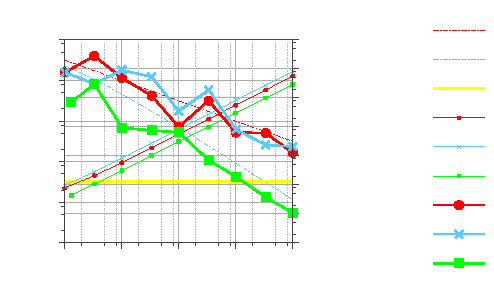
\includegraphics{converge}}%
    \gplfronttext
  \end{picture}%
\endgroup
